\chapter{Http/2}
\label{chap:h2}

\begin{figure}[H]
    \centering
    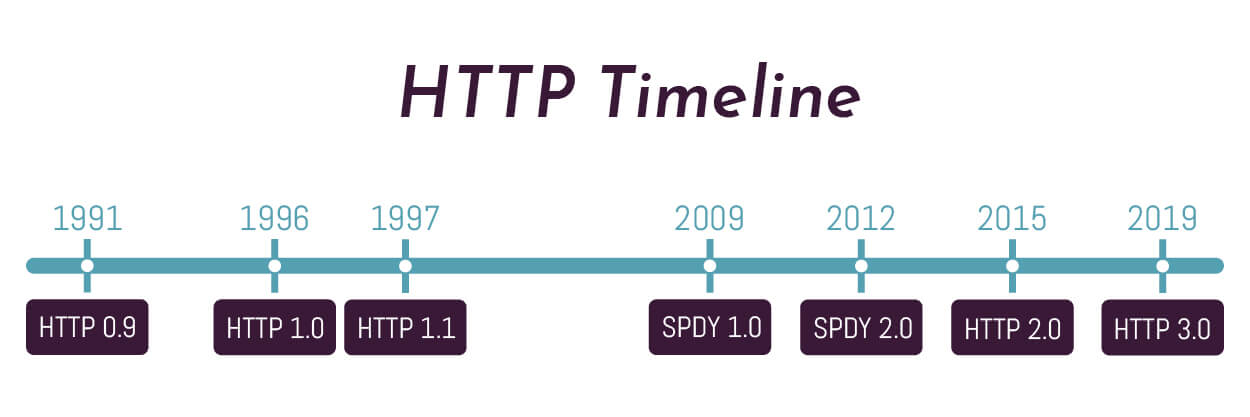
\includegraphics[width=1\textwidth]{http/http_timeline.jpg}
    \caption{HTTP 时间轴}
\end{figure}


\notebox{HTTP标准并未规定TCP就是唯一的传输协议。}


\section{HTTP历史}

\subsection{HTTP/0.9}

\begin{itemize}
    \item 基于TCP协议
    \item 单行请求  GET \qquad 要请求的文档的路径 \qquad  回车符(CRLF)结尾
    \item 连接在文档传输完毕后断开 
\end{itemize}


\subsubsection{重现0.9时代}

\begin{lstlisting}[style=cshell]
    telnet 192.168.31.59 80         # 命令

    Trying 192.168.31.59...
    Connected to 192.168.31.59.

    GET /index.html                 # 命令

    output something... 

    Connection closed by foreign host.
\end{lstlisting}


\begin{figure}[H]
    \centering
    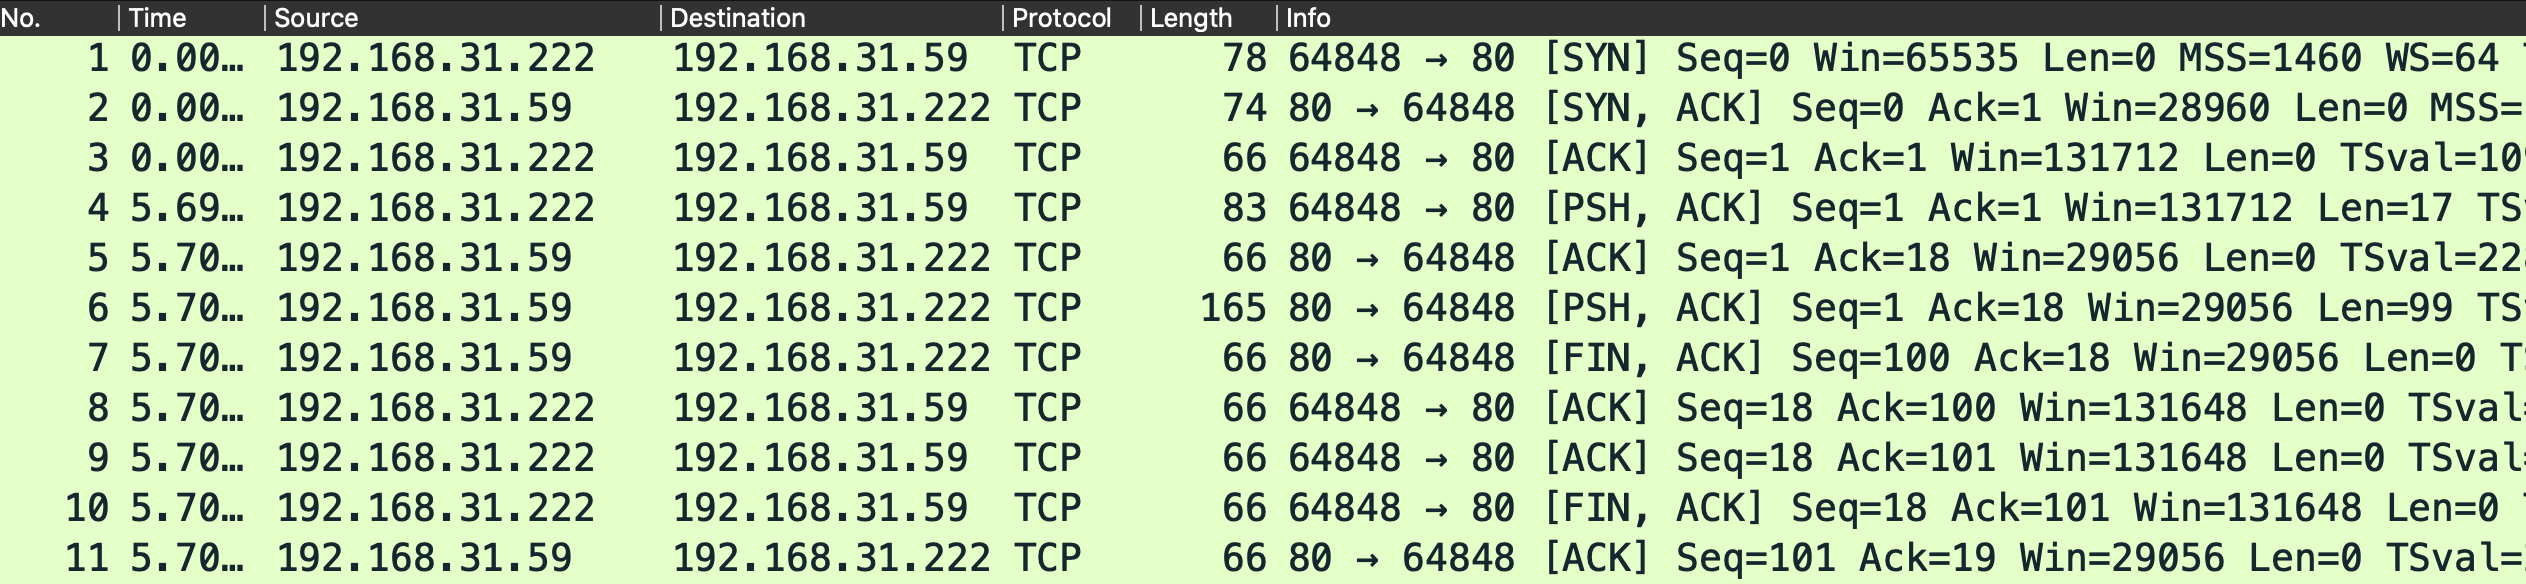
\includegraphics[width=1\textwidth]{http/telnet_http_0_9.png}
    \caption{HTTP/0.9 TCP}
\end{figure}


\begin{figure}[H]
    \centering
    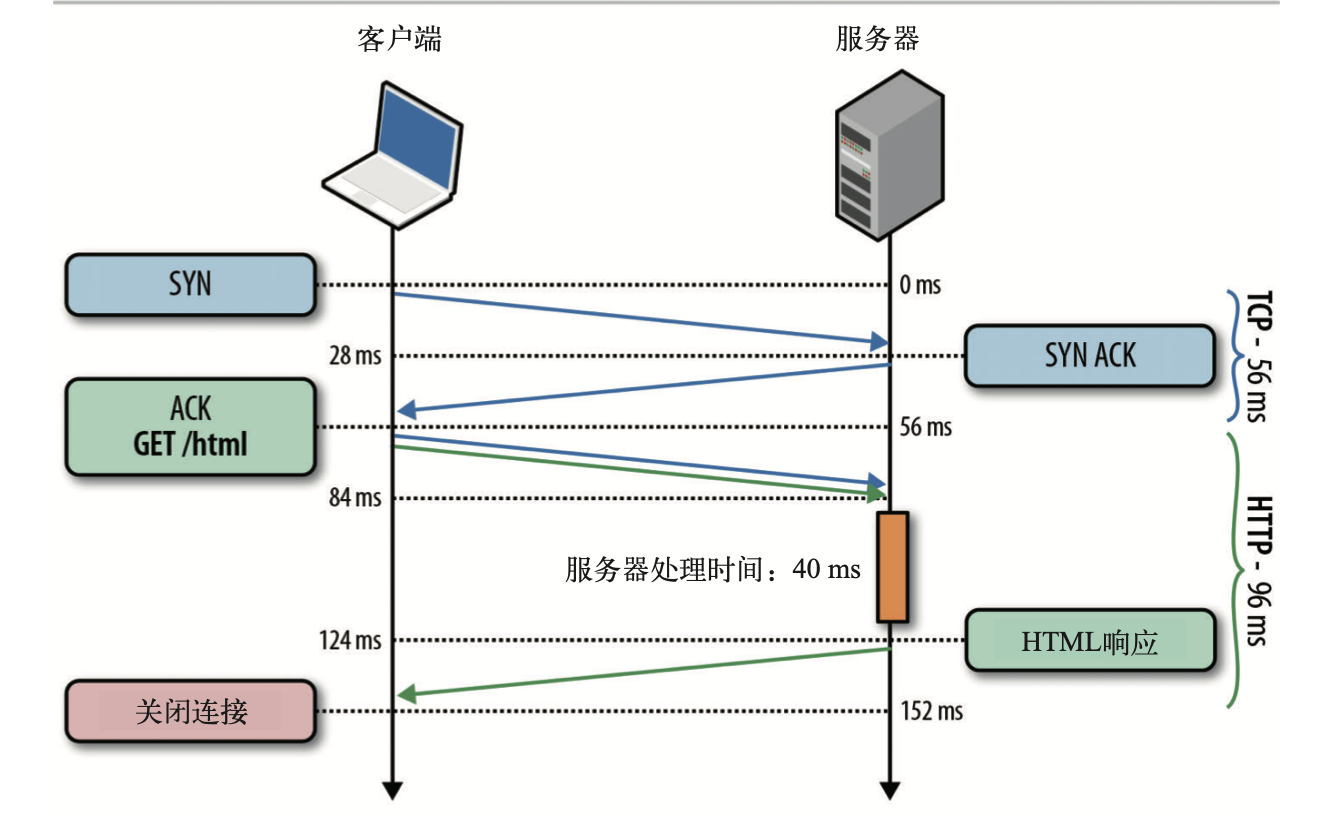
\includegraphics[width=1\textwidth]{http/tcp_http_0_9_flow.png}
    \caption{HTTP/0.9 TCP请求流程图}
\end{figure}





\subsection{HTTP/1.0}

\begin{itemize}
    \item  由起始行、首部、主体构成的请求和响应报文
    \item 响应对象不局限于超文本
    \item 服务器与客户端之间的连接在每次请求之后默认都会关闭
    \item 等等......
\end{itemize}

HTTP/1.0中反向移植了HTTP/1.1持久化连接,通过采用\menlo{Connection: Keep-Alive}可选首部参数。


\subsubsection{重现1.0时代}

\begin{lstlisting}[style=cshell]
    telnet 192.168.31.59 80     # 命令

    Trying 192.168.31.59...
    Connected to 192.168.31.59.

    GET /index.html HTTP/1.0            # 命令
    User-Agent: This is from telnet     # 命令

    HTTP/1.0 200 OK
    Server: nginx/1.10.3 (Ubuntu)
    Date: Thu, 02 Jul 2020 16:36:07 GMT
    Content-Type: text/html
    Content-Length: 99
    Last-Modified: Thu, 02 Jul 2020 16:06:47 GMT
    Connection: close
    ETag: "5efe0617-63"
    Accept-Ranges: bytes

    output something... 

    Connection closed by foreign host.
\end{lstlisting}


\section{HTTP/1.1}

\begin{itemize}
    \item ...... 
    \item 持久连接    persistent connection
    \item 管道化连接   pipeline connection
\end{itemize}


\subsection{持久连接}

* \textbf{在事务处理结束之后仍然保持在打开状态的TCP}

重用对目标服务器打开的空闲持久连接,就可以避免缓慢的连接建立阶段。而且已经打开的连接还可以避免慢启动的拥塞适用阶段。

HTTP/1.1 持久化连接在默认情况下激活的,除非特别指定,否则所有HTTP/1.1所有的连接都是持久化的。如果想要关闭连接需要添加 \menlo{Connection: close}

\begin{figure}[H]
    \centering
    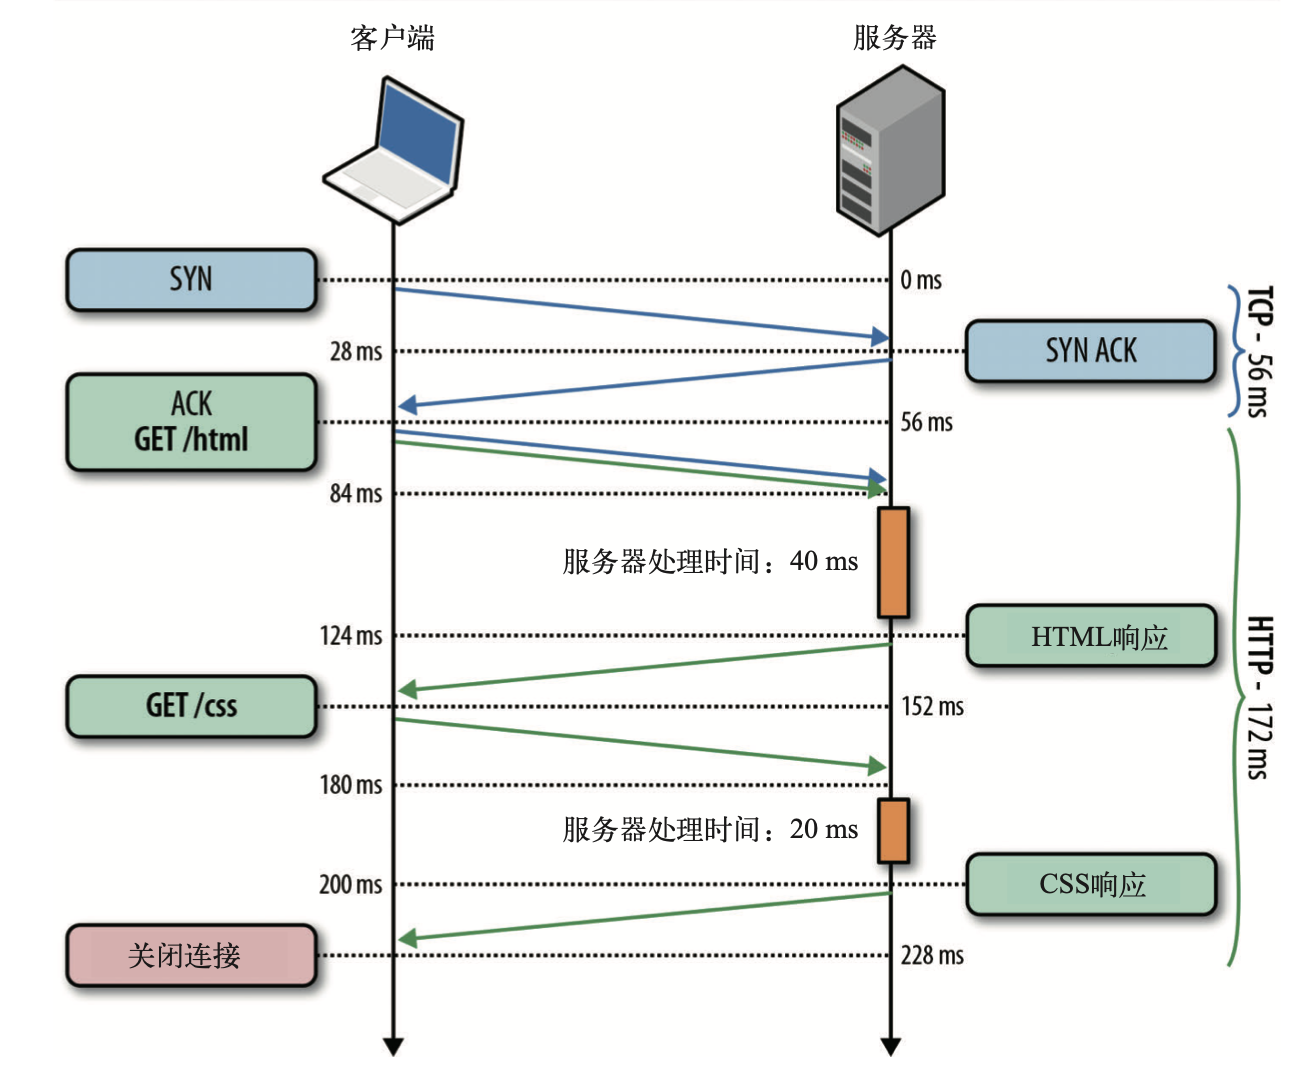
\includegraphics[width=1\textwidth]{http/tcp_http_1_1_persistent_flow.png}
    \caption{HTTP/1.1持久化 TCP请求流程图}
\end{figure}


但是我们的请求还是必须严格按照先进先出(FIFO)的队列顺序:发送请求,等待响应完成,再发送客户端队列中的下一个请求。


\subsection{管道化连接}

\textbf{通过共享的TCP连接发起并发的HTTP请求}

管道化连接是在持久连接的基础上进行的,算是对持久化的优化。把客户端的FIFO队列(请求队列)迁移到服务器(响应队列)。


\begin{figure}[H]
    \centering
    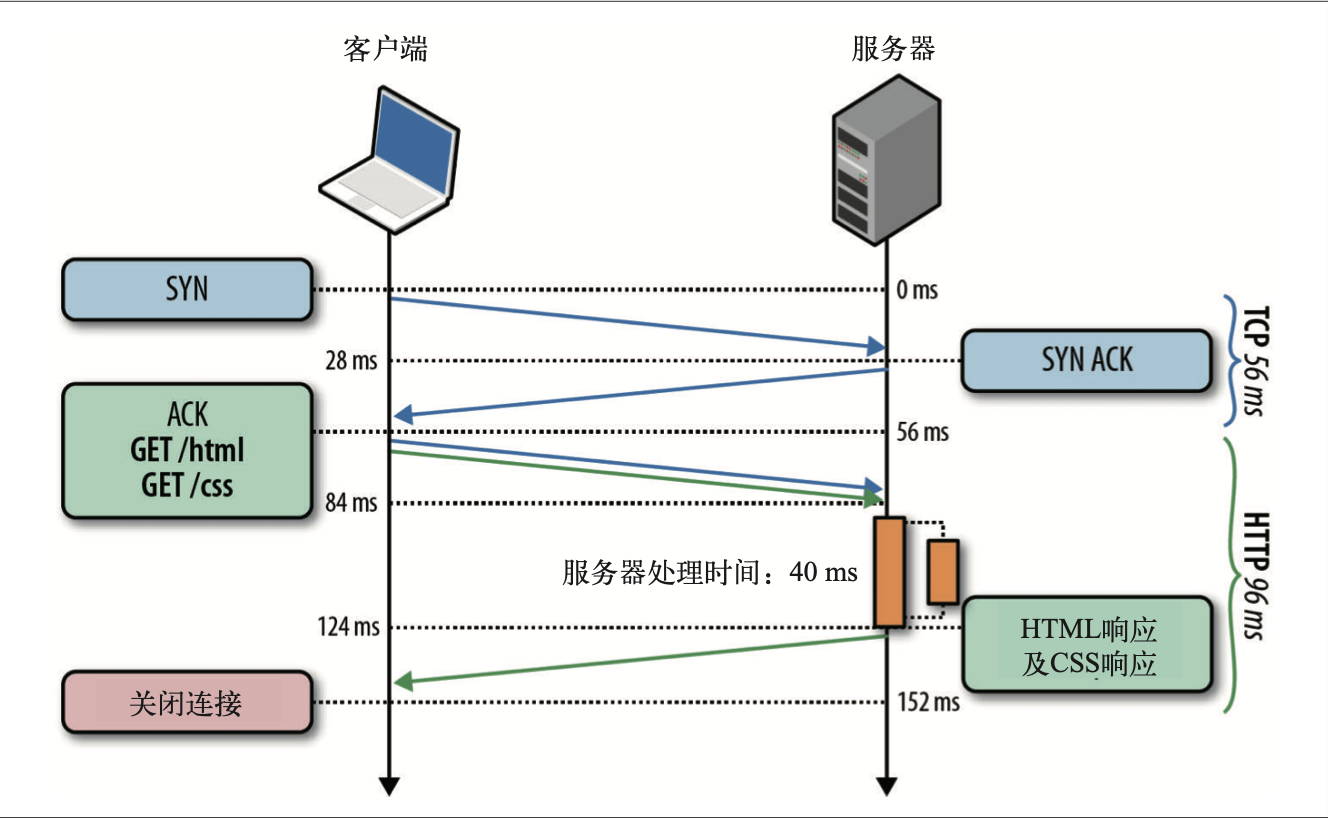
\includegraphics[width=1\textwidth]{http/tcp_http_pipelimne_flow.png}
    \caption{HTTP/1.1持久化 TCP请求流程图}
\end{figure}

严格串行响应,必须按照与请求相同的顺序回送HTTP响应,不支持交错到达(多路复用)

\qquad    HTTP报文中没有序列号标签,如果响应失序了,就没办法与请求匹配了。


按序交付就会导致队首阻塞问题,不能充分利用网络连接,而且会造成服务器缓冲开销等等。

不应该用管道的方式发送非幂等请求

\qquad   例如一系列POST请求,出错的时候我们无法确定那些被正确执行。


目前大部分浏览器是禁用管道技术的。





\subsection{web优化}

并行连接;浏览器默认开启6-8个TCP连接

压缩

缓存

......


\section{HTTP/2}


SPDY(speedy) 是 HTTP 2.0 的基础。

HTTP/2 要解决的问题:

提升性能;

解决HTTP中的“队首阻塞”问题;

并行操作无需与服务器建立多个连接,改进TCP的利用率,尤其是拥塞控制方面;

兼容HTTP/1.1的语义;



\begin{itemize}
    \item One TCP connection
    \item Binary framing layer
    \item Streams and Multiplexing
    \item Header compression (HPACK)
\end{itemize}


\textbf{HTTP/2直观感受}


\href{https://http2.golang.org/gophertiles}{A grid of 180 tiled images is below. Compare}

\subsection{Connection}


\begin{itemize}
    \item   TCP连接三次握手 
    \item   TCP慢启动拥塞控制
    \item   用户捎带确认的TCP延迟确认算法
    \item   TIME\_WAIT时延和端口耗尽
\end{itemize}


HTTP/2两个标识符

\begin{itemize}
    \item h2c
    \item h2
\end{itemize}  

\textbf{h2c}

表示HTTP/2协议运行在明文TCP上。

标识通过明文 TCP 运行 HTTP/2 的协议。此标识符用于 HTTP/1.1 升级标头字段以及标识 HTTP/2 over TCP 的任何位置。

\textbf{h2}

表示 HTTP/2 使用传输层安全性(TLS)TLS的协议。用于 TLS 应用层协议协商(ALPN)。


\subsubsection{通过HTTP Uri启动连接}

发起请求


\begin{lstlisting}[style=cshell]

    GET /index.html HTTP/1.1
    host: nghttp2.org
    connection: Upgrade, HTTP2-Settings
    upgrade: h2c
    http2-settings: AAMAAABkAAQAAP__

\end{lstlisting}


如果不支持HTTP/2,服务忽略h2c 首部字段,返回一个不包含升级的首部响应。

\begin{lstlisting}[style=cshell]

    HTTP/1.1 200 OK
    ...

\end{lstlisting}


如果服务端支持HTTP/2则返回101协议来接受升级请求。101协议响应结束后,服务端开始发送包含HTTP/2帧的请求,第一个被服务端发送的帧是设置帧。
客户端在收到101协议响应后,也发送一个包含设置帧的请求。

\begin{lstlisting}[style=cshell]

HTTP/1.1 101 Switching Protocols
Connection: Upgrade
Upgrade: h2c

\end{lstlisting}


\begin{figure}[H]
    \centering
    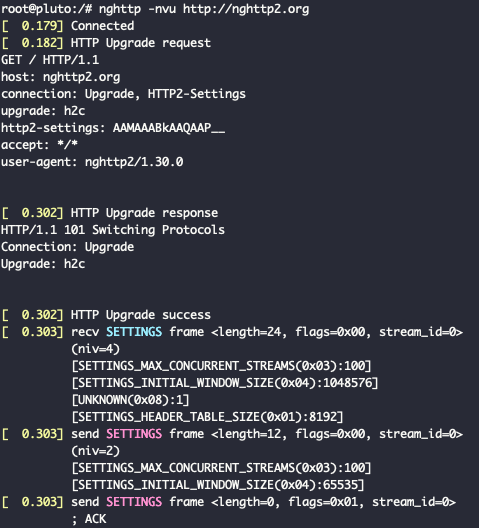
\includegraphics[width=1\textwidth]{http/nghttp_client_http_upgrade.png}
    \caption{nghttp模拟HTTP/1.1 Upgrade}
\end{figure}


\subsubsection{通过HTTPS Uri启动连接}

ALPN(应用层协议协商)

\begin{figure}[H]
    \centering
    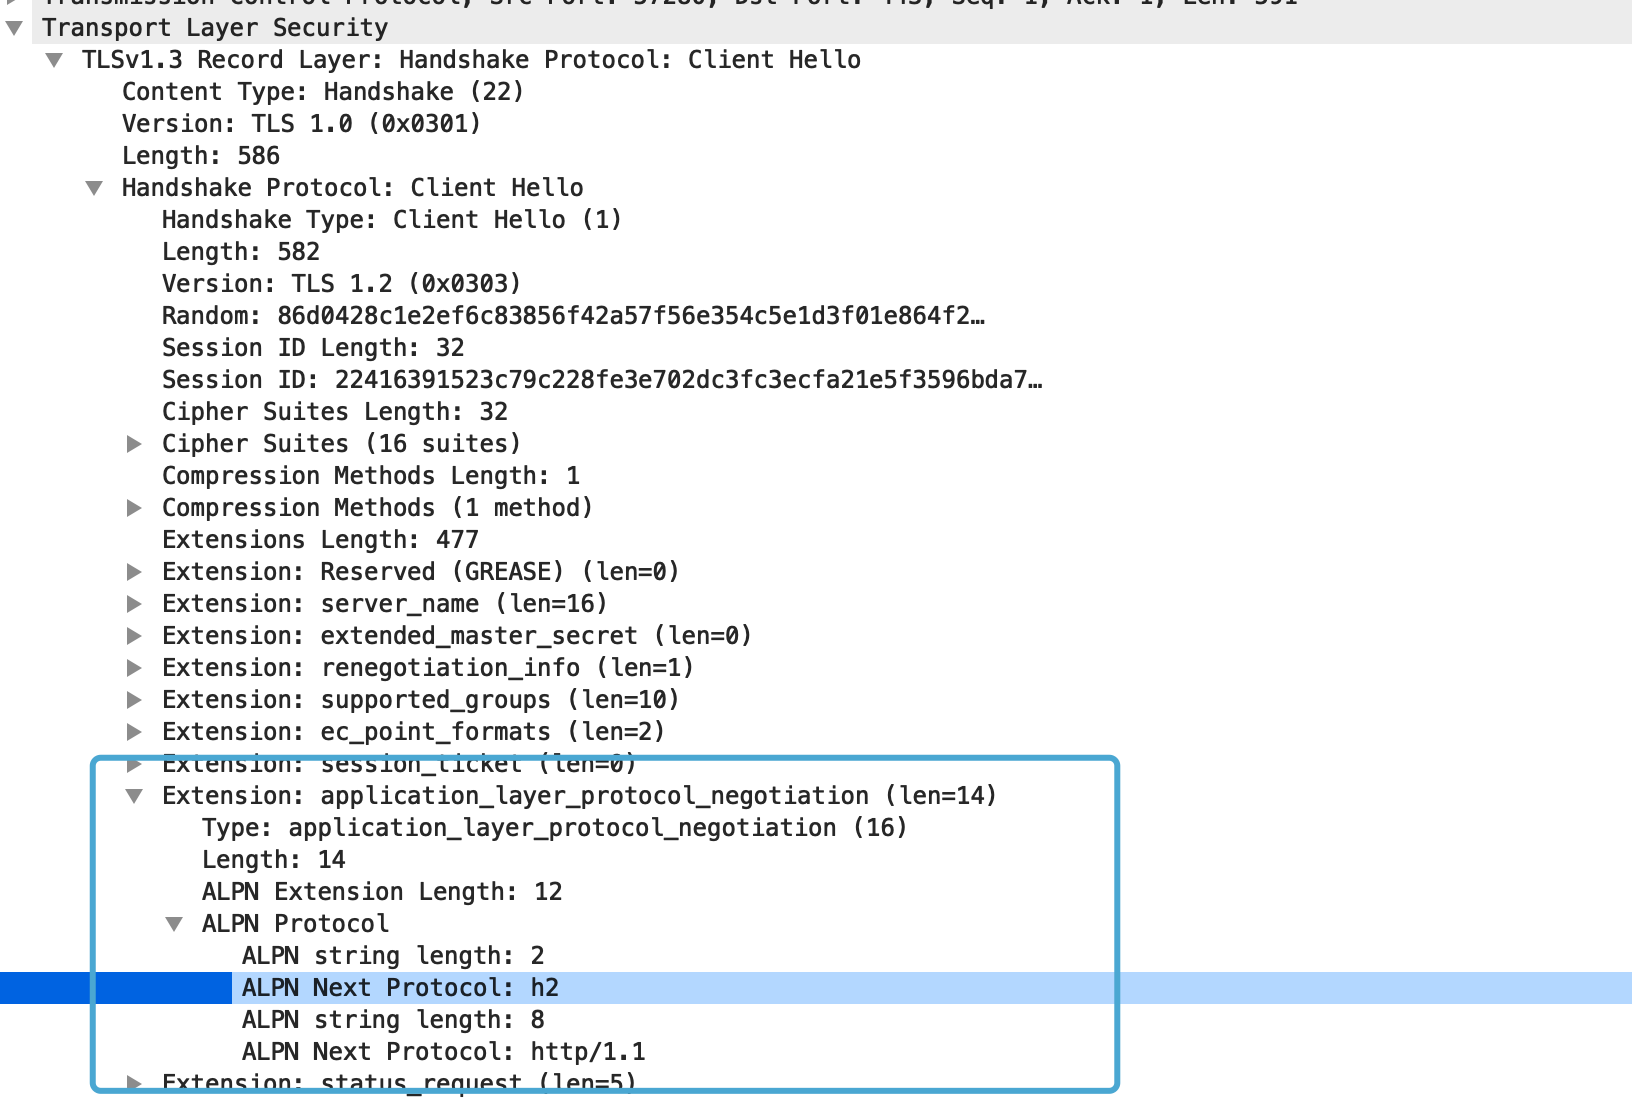
\includegraphics[width=1\textwidth]{http/http_2_client_alpn.png}
    \caption{客户端发起Client Hello协议}
\end{figure}


\begin{figure}[H]
    \centering
    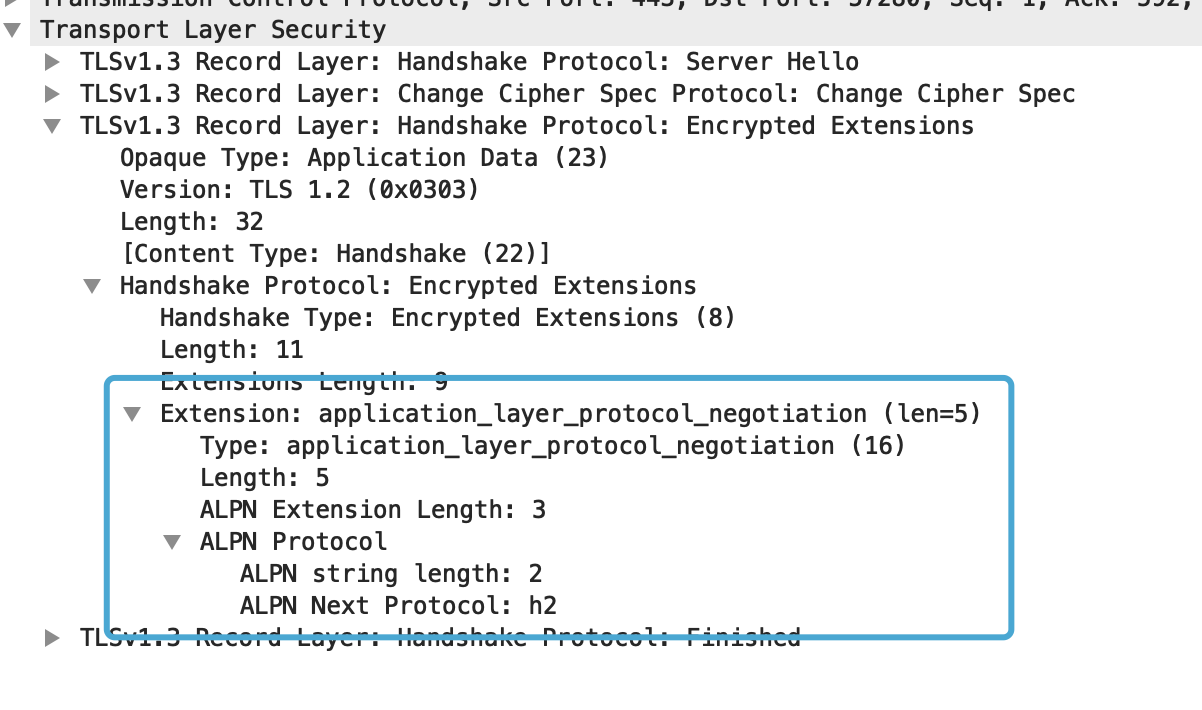
\includegraphics[width=1\textwidth]{http/http_2_server_alpn.png}
    \caption{服务端发起Server Hello协议}
\end{figure}


\subsubsection{HTTP/2 Connection Preface}


在 HTTP/2 中,每个端点都需要发送连接前奏作为正在使用的协议的最终确认,并建立 HTTP/2 连接的初始设置。客户端和服务器各自发送不同的连接前奏。

客户端连接前奏以 24 个八位字节的序列开始,以十六进制表示法为:

\begin{lstlisting}[style=cshell]


0x505249202a20485454502f322e300d0a0d0a534d0d0a0d0a

# 字符串格式: PRI * HTTP/2.0\r\n\r\nSM\r\n\r\n

\end{lstlisting}

该序列必须后跟 可为空的SETTINGS 帧。


服务器连接前奏包含一个可为空的 SETTINGS 帧,该帧必须是服务器在 HTTP/2 连接中发送的第一帧。

服务器可以在客户端发送附加帧之前发送 SETTINGS,从而提供避免此问题的机会。



\begin{figure}[H]
    \centering
    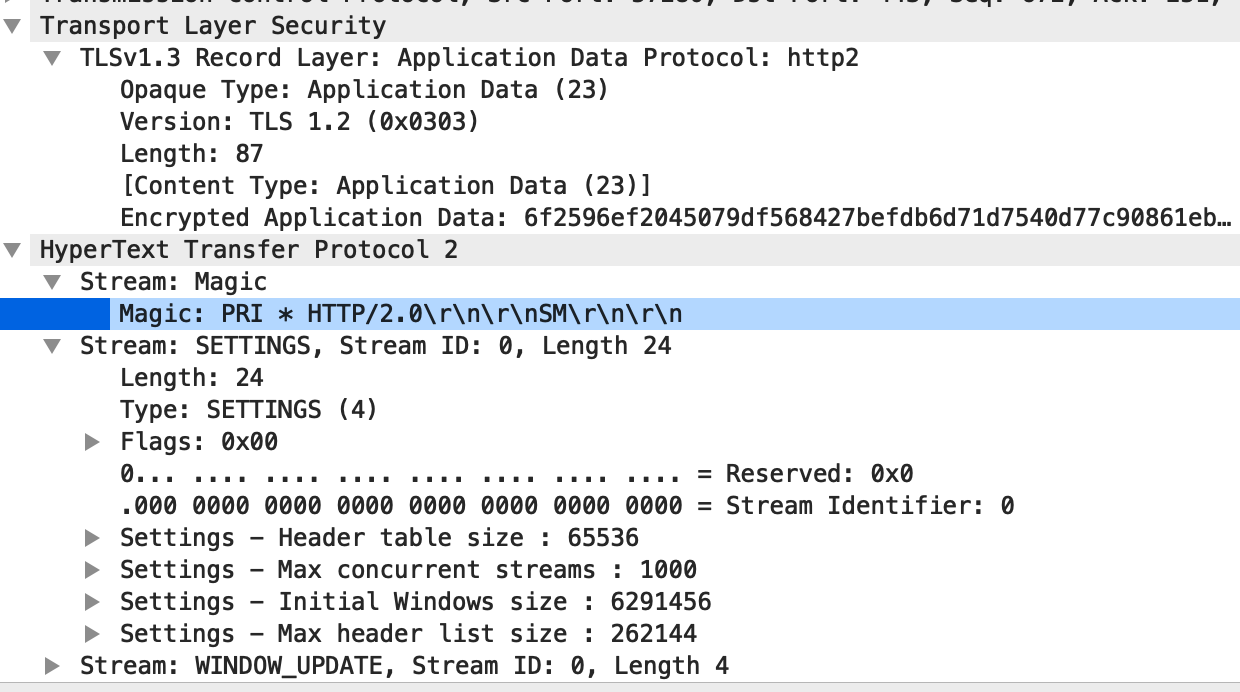
\includegraphics[width=1\textwidth]{http/http_2_connection_preface_prism.png}
    \caption{Connection Preface prism}
\end{figure}


\subsection{Frames}


\begin{figure}[H]
    \centering
    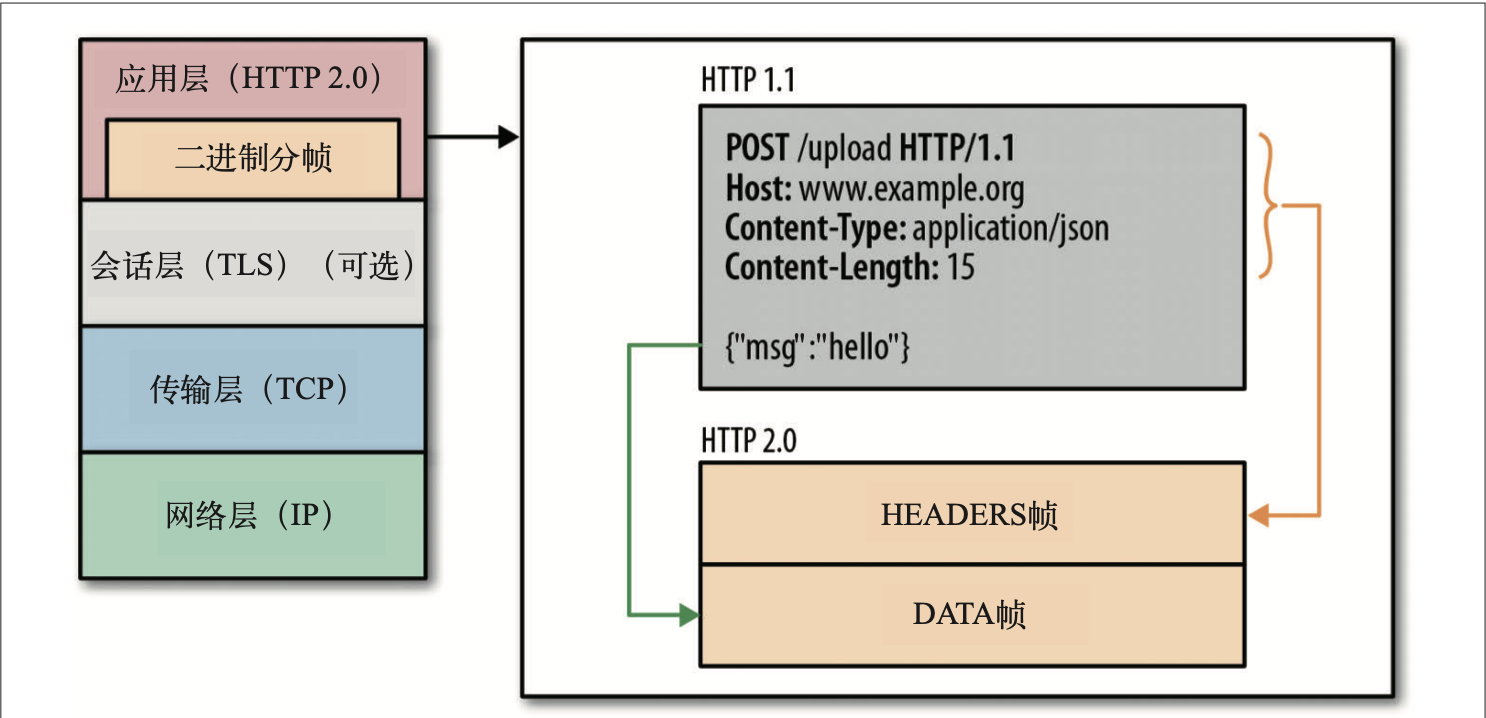
\includegraphics[width=1\textwidth]{http/binary_framing_layer.png}
    \caption{二进制分帧层}
\end{figure}


所有 HTTP 2.0 通信都在一个连接上完成,这个连接可以承载任意数量的双向数据流。
相应地,每个数据流以消息的形式发送,而消息由一或多个帧组成,这些帧可以乱序发送,然后再根据每个帧首部的流标识符重新组装。

HTTP 2.0 的二进制分帧机制解决了 HTTP 1.x 中存在的队首阻塞问题。

\subsubsection{Frame Layout}

帧就是HTTP 2.0 通信的最小单位,每个帧包含帧首部,至少也会标识出当前帧所属的流。

\begin{figure}[H]
    \centering
    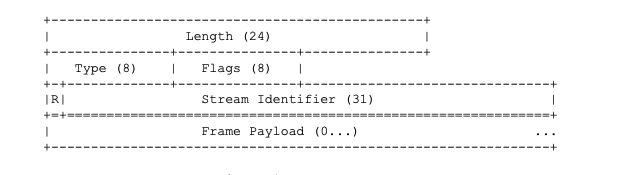
\includegraphics[width=1\textwidth]{http/frame_layout.png}
    \caption{HTTP/2帧结构}
\end{figure}


\begin{table}[H]
    \renewcommand{\arraystretch}{2}
    \centering
    \begin{tabular} {p{70pt}p{50pt}p{250pt}}
    \hline
    名称                 & 长度      &   描述                                      \\ \hline
    Length              & 3字节     &   表示帧负载的长度(取值范围为$2^{14}$ $\sim$ $2^{24}$-1)。默认最大帧大小是$2^{14}$。可以通过SETTINGS帧修改。            \\ \hline
    Type                & 1字节     &   当前帧类型                                  \\ \hline
    Flags               & 1字节     &   具体帧类型的标识                            \\ \hline
    R                   & 1位       &   保留位                                    \\ \hline
    Stream Identifier    & 31位      &   每个流的唯一ID                             \\ \hline
    Frame Payload       & 长度可变   &   真实帧内容;长度设置在Length中               \\ \hline
    \end{tabular}
    \caption{\label{tab:table-name}帧字段}
    \end{table}


    前9个字节是帧的固定结构。解析时只需要读取这些字节。



\begin{table}[H]
    \renewcommand{\arraystretch}{1.5}
    \centering
     \begin{tabular} {p{100pt}p{30pt}p{250pt}}
     \hline
    名称             & ID      &   描述                             \\ \hline
    DATA            & 0x0     &   流核心内容                          \\ \hline
    HEADERS         & 0x1     &  HTTP首部以及可选的优先级参数           \\ \hline
    PRIORITY        & 0x2     &  指示或者更改流的优先级和依赖           \\ \hline
    RST\_STREAM     & 0x3     &  允许一段停止流(通常由于错误导致的)     \\ \hline
    SETTINGS        & 0x4     &  协商连接级参数                       \\ \hline
    PUSH\_PROMISE   & 0x5     &  提示客户端,服务器要推送东西            \\ \hline
    PING            & 0x6     &  测试连接可用性和往返时延(RTT)           \\ \hline
    GOAWAY          & 0x7     &  告诉另一段,当前端已结束                \\ \hline
    WINDOW\_UPDATE  & 0x8     &  用于流量控制;协商一段将要接受多少字节     \\ \hline
    CONTINUATION    & 0x9     &  用以扩展HEADER数据块                   \\ \hline
    \end{tabular}
    \caption{\label{tab:table-name}帧类型}
    \end{table}


\subsubsection{DATA}

\begin{figure}[H]
    \centering
    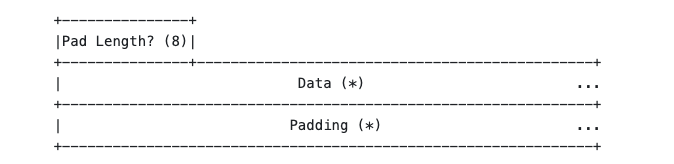
\includegraphics[width=1\textwidth]{http/data_frame_payload.png}
    \caption{DATA帧结构}
\end{figure}

DATA 帧包含以下几个字段:

Pad Length:
一个 8 位字段,包含以八位字节为单位的帧填充长度。该字段是有条件的,仅在设置了 PADDED 标志时才存在。

Data:
应用数据。在减去存在的其他字段的长度之后,data 的大小是帧有效载荷的剩余部分。

Padding:
填充的八位字节,它不包含应用程序语义值。发送时,填充的八位字必须设置为零。接收方没有义务验证填充,但可以将非零填充视为 PROTOCOL\_ERROR 类型的连接错误。


DATA 帧定义了以下 flag 标识:

END\_STREAM (0x1):
设置这个字段的时候,位 0 表示该帧是端点为将要发送的标识流的最后一帧。设置此标志会导致流进入"半关闭"状态或者"关闭"状态。

PADDED (0x8):
设置这个字段的时候,位 3 表示存在 Pad Length 字段及其描述的任何填充。


\begin{figure}[H]
    \centering
    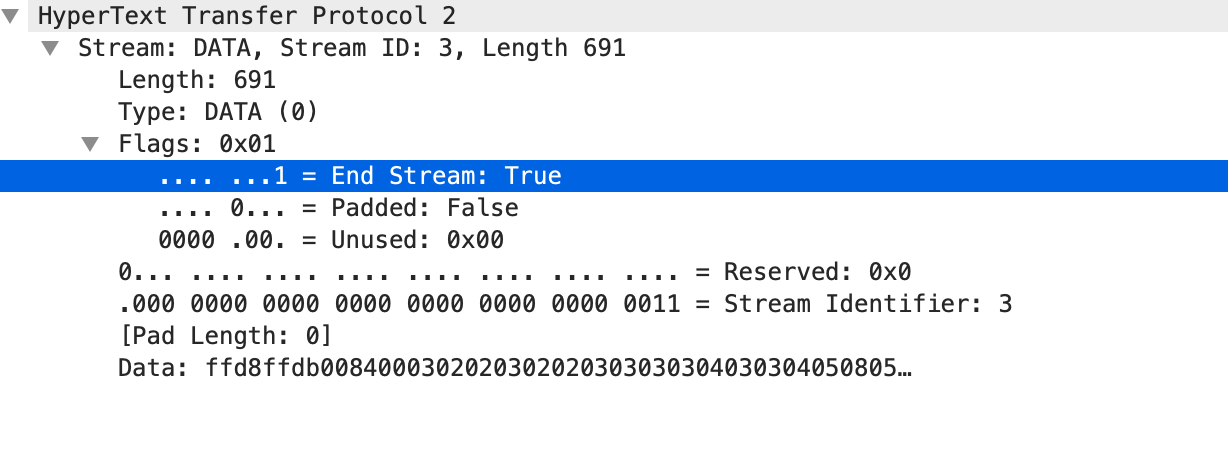
\includegraphics[width=1\textwidth]{http/data_frame_end_stream_flags.png}
    \caption{END\_STREAM}
\end{figure}



DATA 帧必须与某一个流相互关联。如果接收到其流标识符字段为 0x0 的 DATA 帧,则接收方必须以 PROTOCOL\_ERROR 类型的连接错误进行响应。

DATA 帧会受到流量控制,只能在流处于“打开”或“半关闭(远程)”状态时发送。整个 DATA 帧有效载荷包含在流量控制中,包括 Pad Length 和 Padding 字段(如果存在)。如果收到的数据帧的流不是“打开”或“半关闭(本地)”状态,则接收方必须以 STREAM\_CLOSED 类型的流错误进行响应。

填充八位字节的总数由填充长度字段的值确定。如果填充的长度是帧有效负载的长度或更长,则接收方必须将其视为 PROTOCOL\_ERROR 类型的连接错误。


\subsubsection{HEADERS}

\begin{figure}[H]
    \centering
    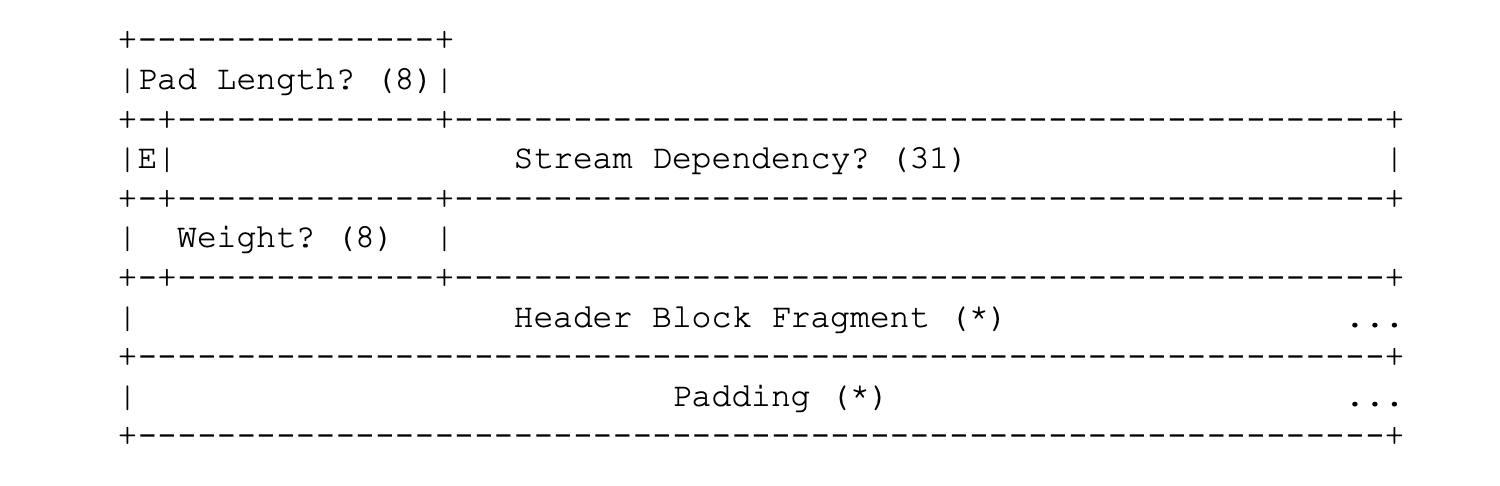
\includegraphics[width=1\textwidth]{http/headers_frame_payload.png}
    \caption{HEADERS帧结构}
\end{figure}


Pad Length: 指定 Padding 长度,存在则代表 PADDING flag 被设置

E: 一个比特位声明流的依赖性是否是排他的,存在则代表 PRIORITY flag 被设置

Stream Dependency: 指定一个 stream identifier,代表当前流所依赖的流的 id,存在则代表 PRIORITY flag 被设置

Weight: 一个无符号 8 为整数,代表当前流的优先级权重值 (1~256),存在则代表 PRIORITY flag 被设置

Header Block Fragment: header 块片段

Padding: 填充字节,没有具体语义,作用与 DATA 的 Padding 一样,存在则代表 PADDING flag 被设置

HEADERS 帧有以下标识 (flags):

END\_STREAM: bit 0 设为 1 代表当前 header 块是发送的最后一块,但是带有 END\_STREAM 标识的 HEADERS 帧后面还可以跟 CONTINUATION 帧 (这里可以把 CONTINUATION 看作 HEADERS 的一部分)

END\_HEADERS: bit 2 设为 1 代表 header 块结束

PADDED: bit 3 设为 1 代表 Pad 被设置,存在 Pad Length 和 Padding

PRIORITY: bit 5 设为 1 表示存在 Exclusive Flag (E), Stream Dependency, 和 Weight


\begin{figure}[H]
    \centering
    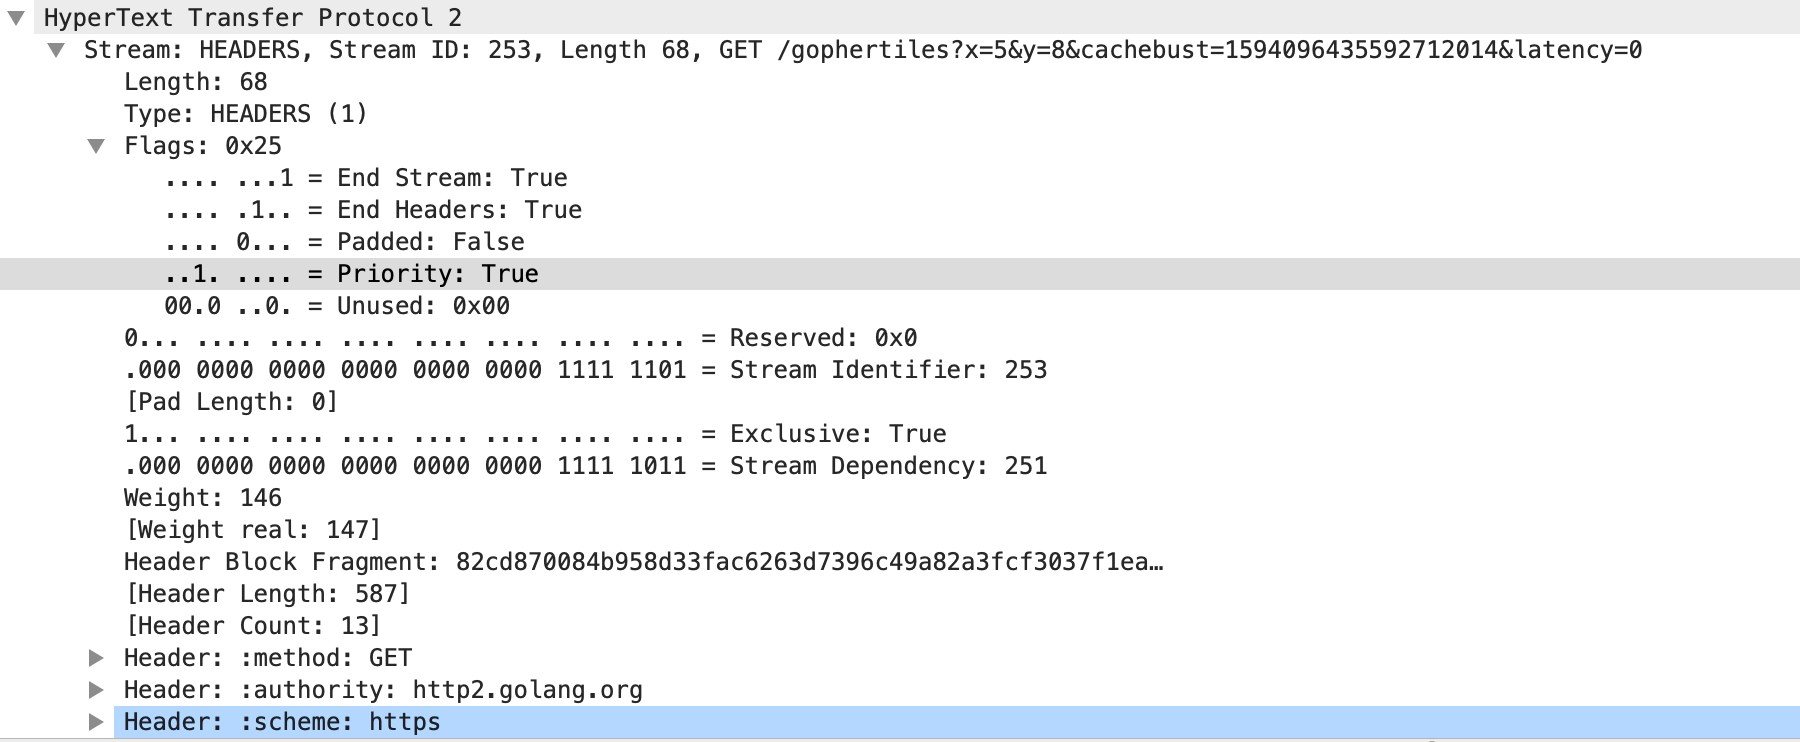
\includegraphics[width=1\textwidth]{http/http_2_headers_frame_flags.png}
    \caption{HEADERS帧结构}
\end{figure}



\subsubsection{SETTINGS}

\begin{figure}[H]
    \centering
    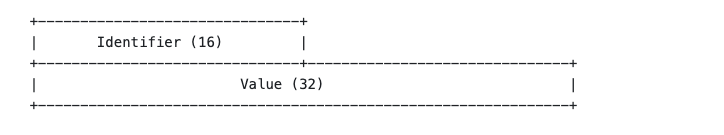
\includegraphics[width=1\textwidth]{http/http_2_setting_format.png}
    \caption{SETTINGS帧结构}
\end{figure}

SETTINGS\_HEADER\_TABLE\_SIZE(0x1)

SETTINGS\_ENABLE\_PUSH(0x2)

SETTINGS\_MAX\_CONCURRENT\_STREAMS(0x3)

SETTINGS\_INITIAL\_WINDOW\_SIZE(0x4)

SETTINGS\_MAX\_FRAME\_SIZE(0x5)

SETTINGS\_MAX\_HEADER\_LIST\_SIZE(0x6)


\subsection{Stream}

HTTP/2连接上独立的,双向的帧序列交换。

\begin{figure}[H]
    \centering
    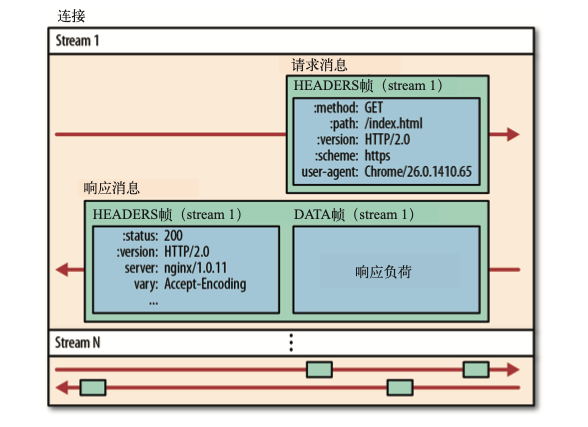
\includegraphics[width=1\textwidth]{http/http_2_frame.png}
    \caption{流、消息和帧}
\end{figure}

客户端到服务端的h2连接建立之后,通过发送HEADERS帧来启动新的流,如果首部需要跨多个帧,可能还会发送CONTINUATION帧。
后续流启动会发送一个带有自增Stream Identifier的新HEADERS帧。

\notebox{HEADERS和CONTINUATION帧必须是有序的。}


stream 流使用无符号的 31 位整数标识。
由客户端发起的流必须使用奇数编号的流标识符。

服务器发起的必须使用偶数编号的流标识符。

流标识符零(0x0)用于连接控制消息;零流标识符不能用于建立新的 stream 流。

HTTP/1.1 Upgrade to HTTP/2 时响应的流 ID 是 0x1,在升级完成之后,流 0x1 在客户端会转为 half-closed (local) 状态,因此这种情况下客户端不能用 0x1 初始化一个流。
因为HTTP/1.1请求已经完成了。


\subsubsection{流生命周期}

\begin{figure}[H]
    \centering
    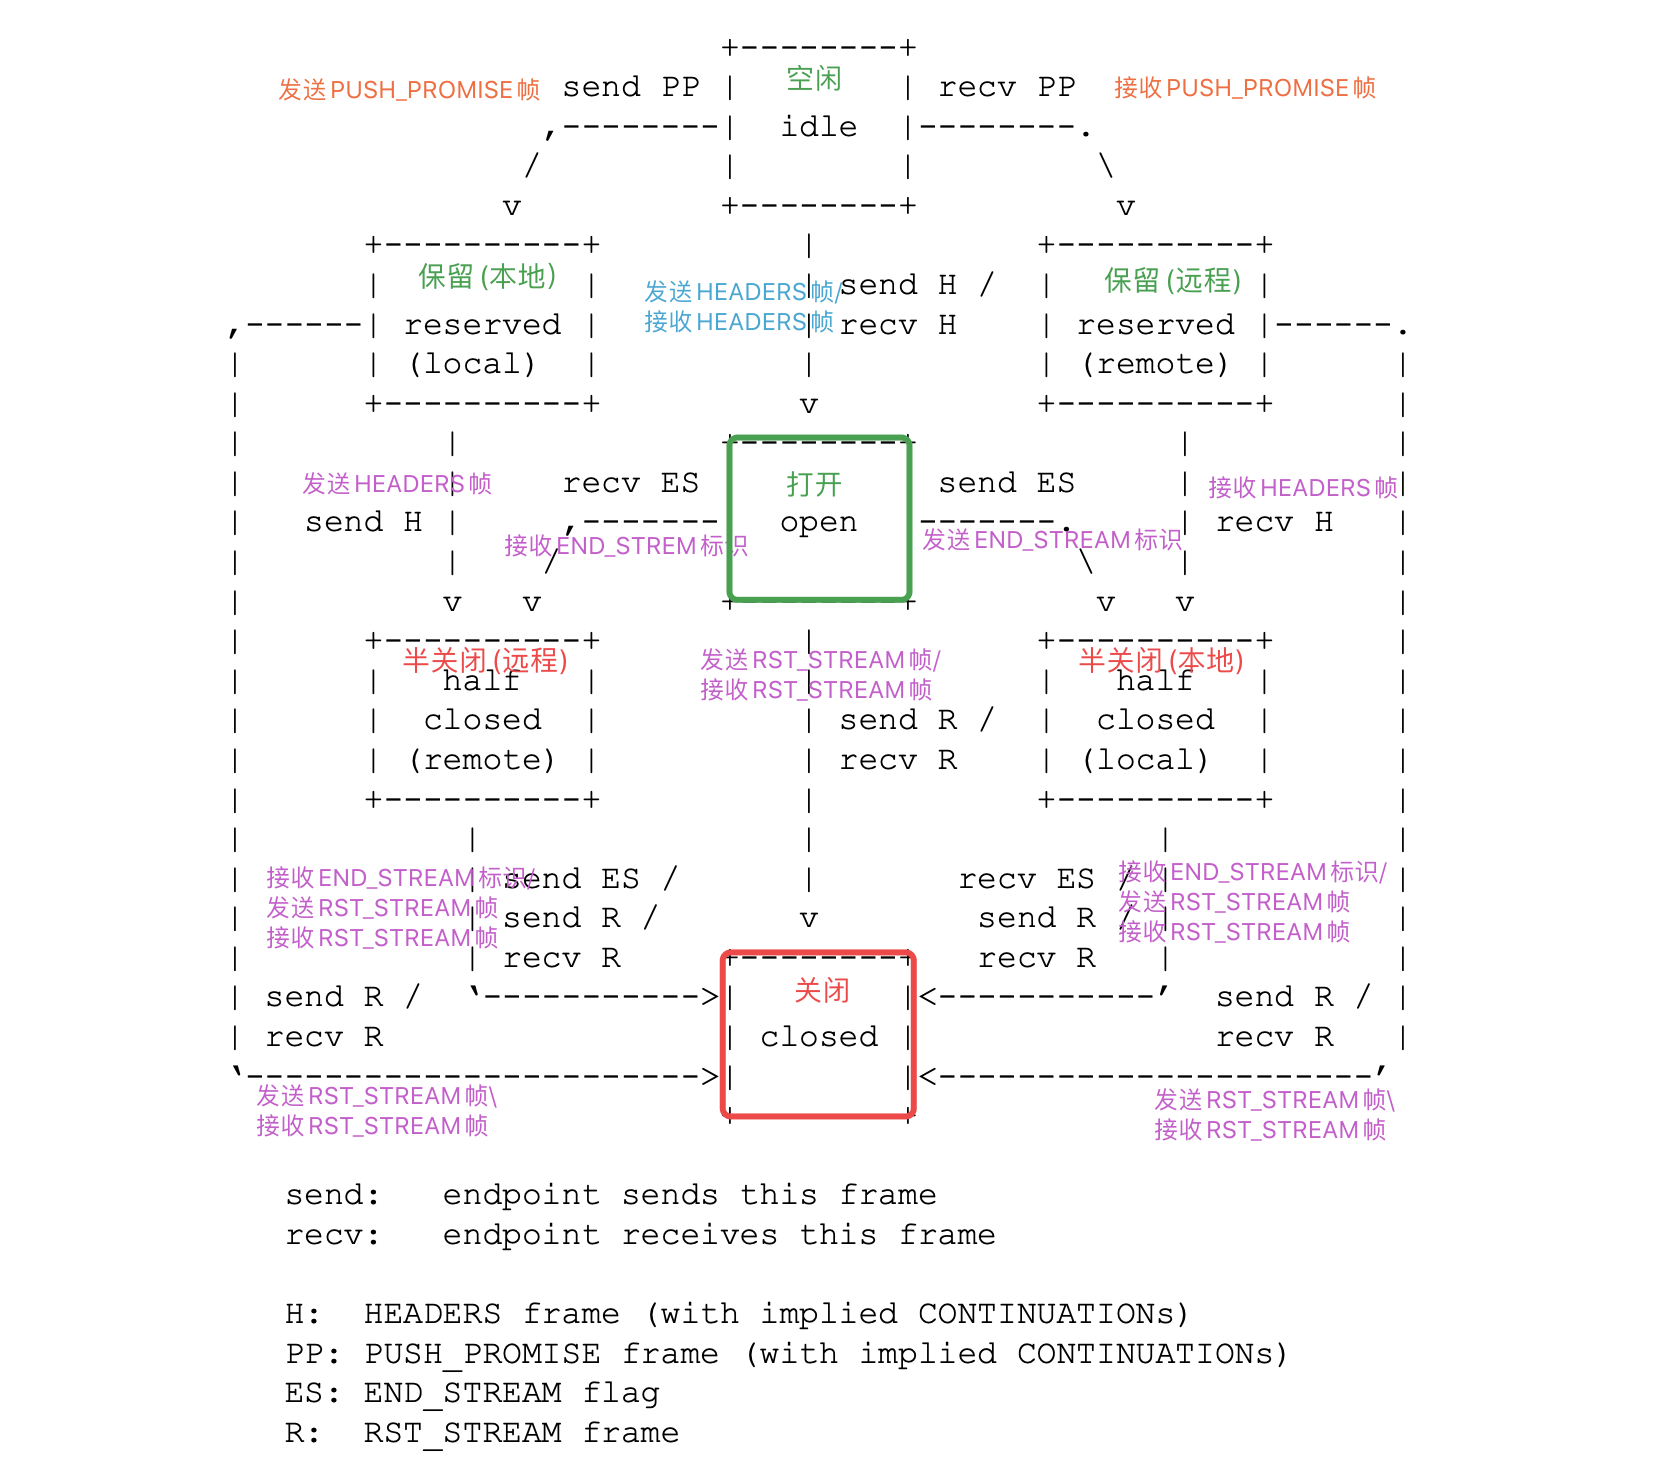
\includegraphics[width=1\textwidth]{http/stream_life.png}
    \caption{流生命周期}
\end{figure}


\textbf{idle}

所有的 stream 流都是从空闲态开始的。

\textbf{reserved}

reserved,为推送保留一个流稍后使用。

reserved(local)

\qquad 服务器端发送完PUSH\_PROMISE帧本地预留的一个用于推送流所处于的状态

\qquad 只能发送HEADERS、RST\_STREAM、PRIORITY帧

\qquad 只能接收RST\_STREAM、PRIORITY、WINDOW\_UPDATE帧

reserved(remote)

\qquad 客户端接收到PUSH\_PROMISE帧,本地预留的一个用于接收推送流所处于的状态

\qquad 只能发送WINDOW\_UPDATE、RST\_STREAM、PRIORITY帧

\qquad 只能接收RST\_STREAM、PRIORITY、HEADERS帧

\qquad 不满足条件,需要报PROTOCOL\_ERROR类型连接错误


\textbf{open}

\qquad 用于两端发送帧,需要发送数据的对等端需要遵守流量控制的通告。

\qquad 每一端可以发送包含END\_STREAM标志位的帧,导致流进入"half closed"状态

\qquad 每一端都可以发送RST\_STREAM帧,流进入"closed"状态


 \textbf{half closed}

 half closed(local)

 发送包含有END\_STREAM标志位帧的一端,流进入本地半关闭状态

 \qquad 不能发送WINDOW\_UPDATE,PRIORITY和RST\_STREAM帧

 \qquad 可以接收到任何类型帧

 \qquad 接收者可以忽略WINDOW\_UPDATE帧,后续可能会马上接收到包含有END\_STREAM标志位帧

 \qquad 接收到优先级PRIORITY帧,可用来变更依赖流的优先级顺序

 \qquad 一旦接收到包含END\_STREAM标志位的帧,将进入"closed"状态

 half closed(remote)
 
接收到包含有END\_STREAM标志位帧的一端,流进入远程半关闭状态
 
    \qquad 对流量控制窗口可不用维护

    \qquad 只能接收RST\_STREAM、PRIORITY、WINDOW\_UPDATE帧,否则报STREAM\_CLOSED流错误

    \qquad 终端可以发送任何类型帧,但需要遵守对端的当前流的流量控制限制

    \qquad 一旦发送包含END\_STREAM标志位的帧,将进入"closed"状态

一旦接收或发送RST\_STREAM帧,流将进入"closed"状态

\textbf{closed}

流的最终关闭状态



\begin{figure}[H]
    \centering
    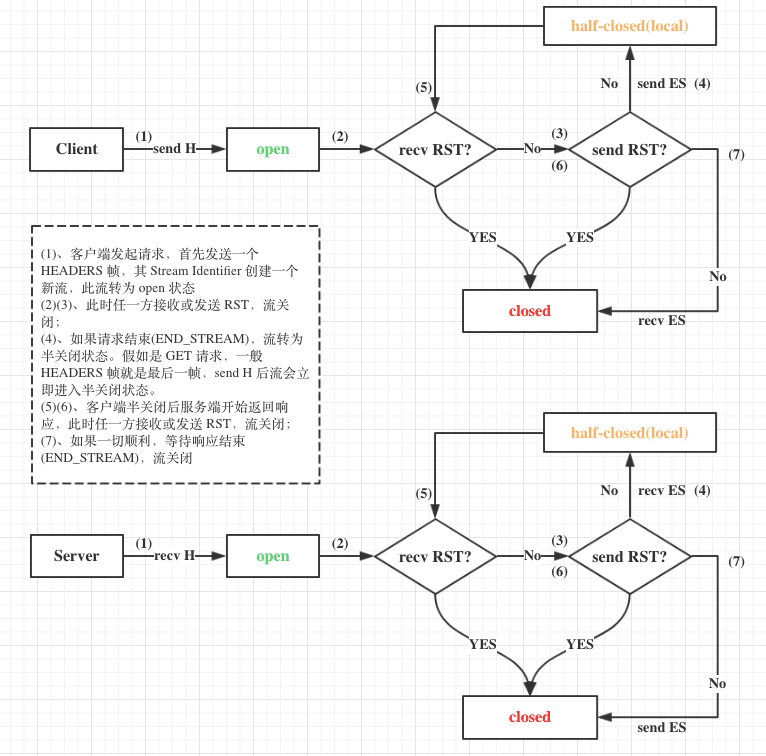
\includegraphics[width=1\textwidth]{http/http_2_request_stream.png}
    \caption{请求/响应流状态态转化}
\end{figure}

\begin{figure}[H]
    \centering
    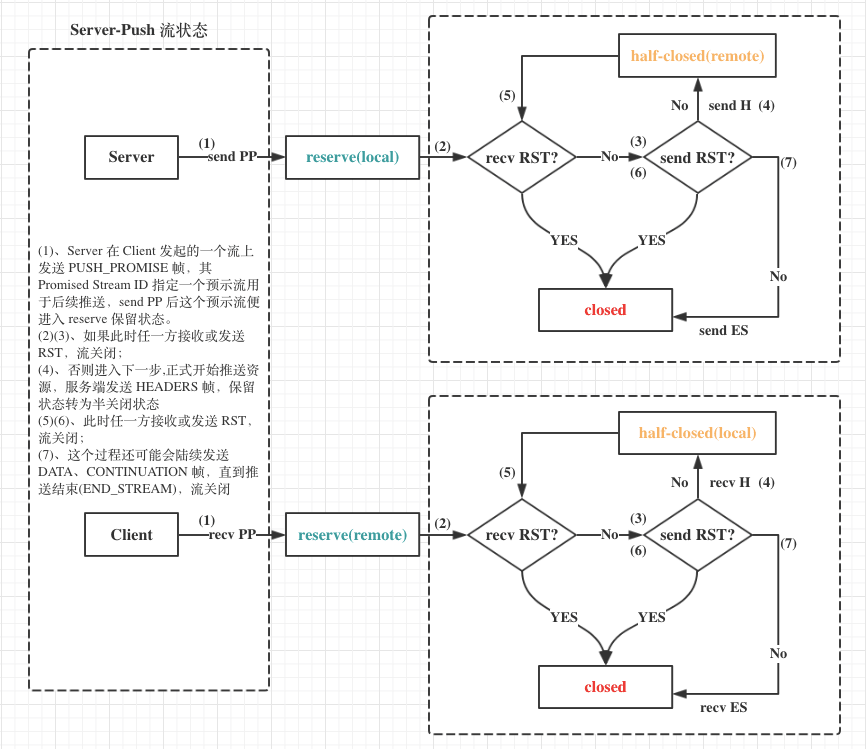
\includegraphics[width=1\textwidth]{http/http_2_server_push.png}
    \caption{Server Push}
\end{figure}


\subsubsection{流优先级}

\begin{itemize}
    \item 依赖关系
    \item 权重
\end{itemize} 


客户端可以通过在打开流的 HEADERS 帧中包含优先级信息来为新的流分配优先级。在任何其他时间,PRIORITY 帧可用于更改流的优先级。

确定优先级的目的是允许端点在管理并发流时表达它希望其对端如何分配资源。最重要的是,当发送容量有限时,可以使用优先级来选择用于发送帧的流。

可以通过将流标记为依赖其他流的完成,来确定流的优先级。为每个依赖项分配一个相对权重,该数字用于确定分配给依赖于相同流的 stream 流的可用资源的相对比例。


\begin{figure}[H]
    \centering
    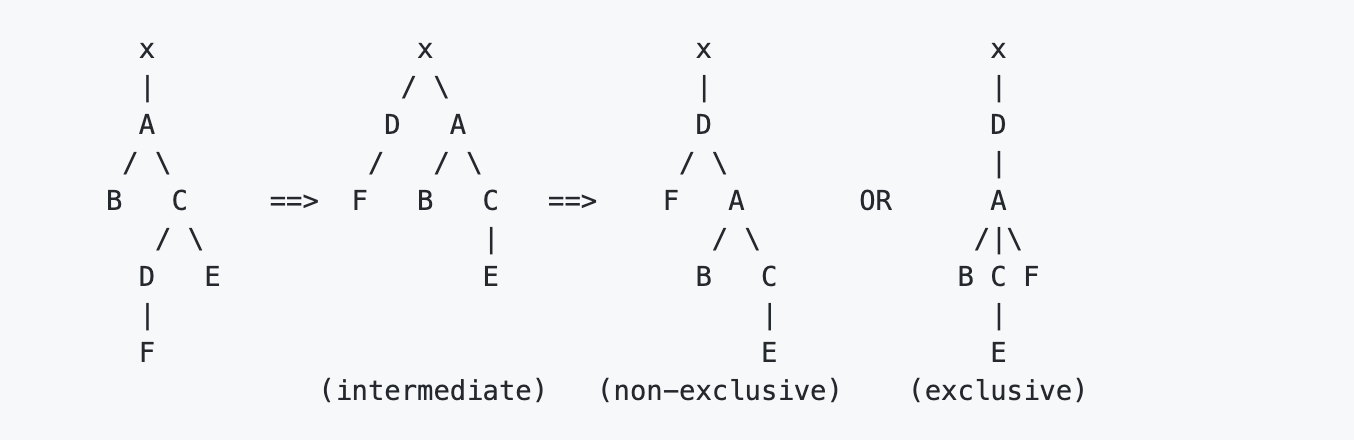
\includegraphics[width=1\textwidth]{http/http_2_dependency_reprioritization.png}
    \caption{依赖优先级调整}
\end{figure}

D 优先级变高


\begin{figure}[H]
    \centering
    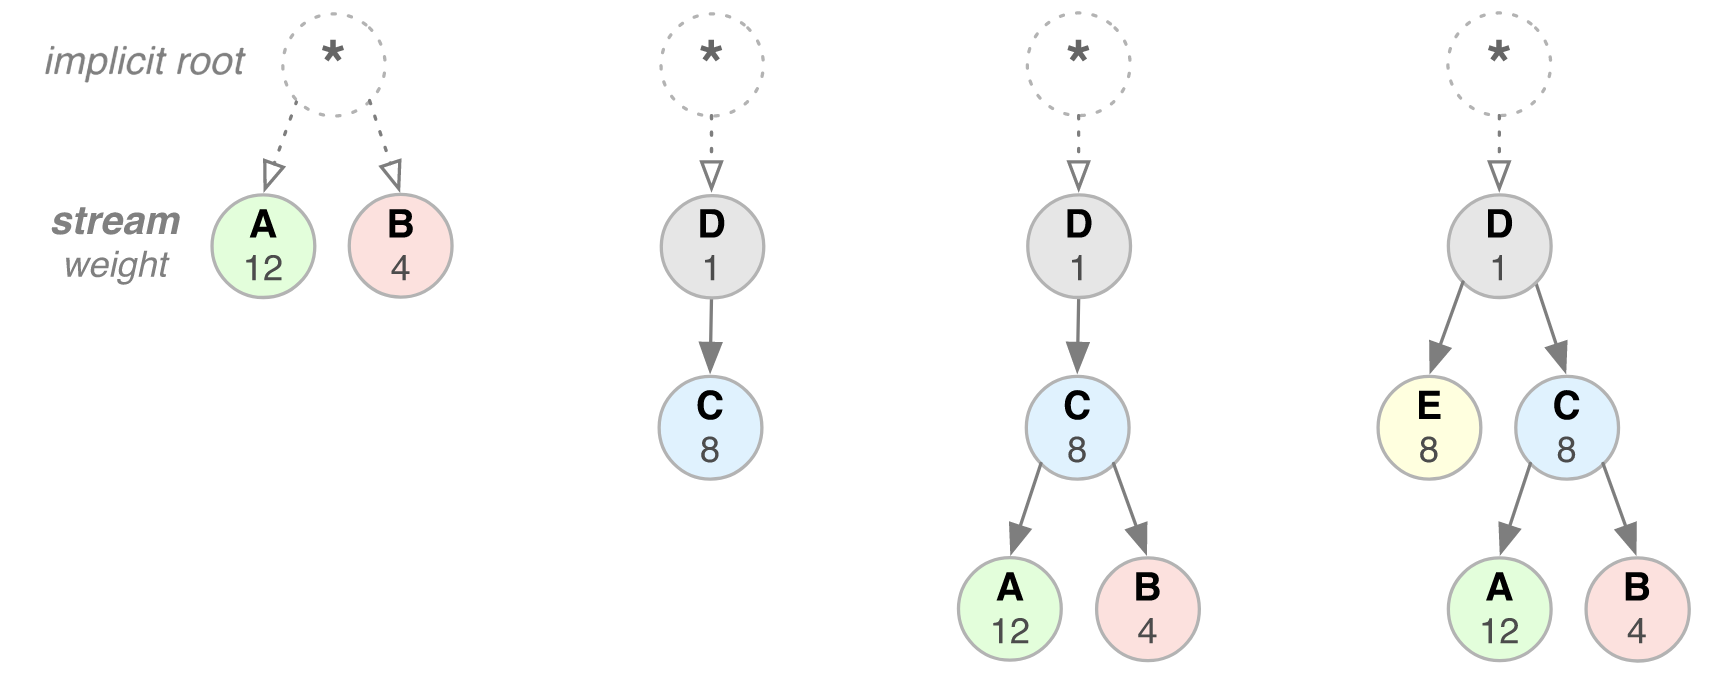
\includegraphics[width=1\textwidth]{http/http_2_dependency_weighting.png}
    \caption{依赖以及权重}
\end{figure}


\subsubsection{流量控制}

HTTP/2 通过使用 WINDOW\_UPDATE 帧提供流量控制

只有 DATA 帧受流量控制

流控制窗口的默认值设为 65,535 字节

\begin{figure}[H]
    \centering
    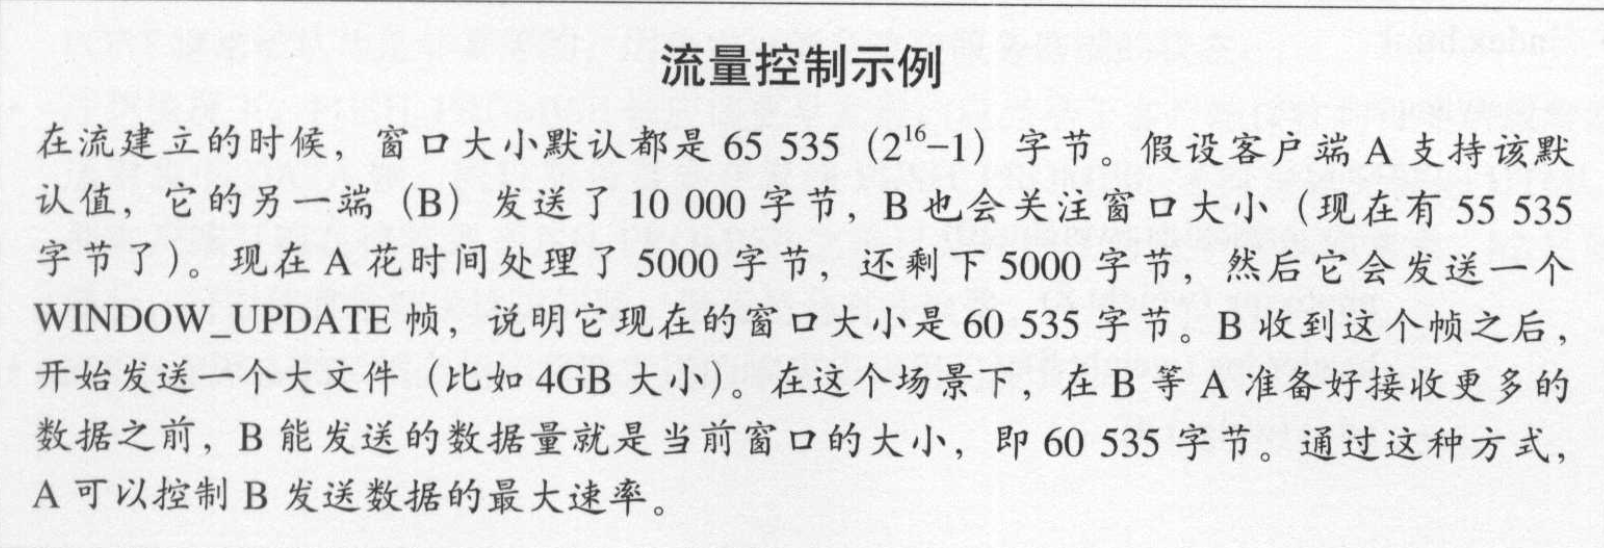
\includegraphics[width=1\textwidth]{http/http_2_flow_control_demo.png}
    \caption{流量控制示例}
\end{figure}


\subsubsection{服务器推送}

\href{https://www.nginx.com/blog/nginx-1-13-9-http2-server-push/}{http2-server-push}


\section{HPACK}

\subsection{Deflate}

LZ77 + Huffman

CRIME漏洞

攻击者在请求中(cookie)添加数据,观察压缩加密后的数据量是否会小于预期,如果变小了,注入的文本和请求中的其他内容有重复。


\subsection{Huffman Coding}

\href{https://people.ok.ubc.ca/ylucet/DS/Huffman.html}{动画演示}

\subsection{索引表}

静态表(Static Table)和动态表(Dynamic Table)

\textbf{}{静态表}

静态索引表由预定义的首部字段构成。包含61个预定义Header key-value。

\href{https://tools.ietf.org/html/rfc7541#appendix-A}{静态索引表字段}


\textbf{动态表}

\subsection{实现}

\begin{figure}[H]
    \centering
    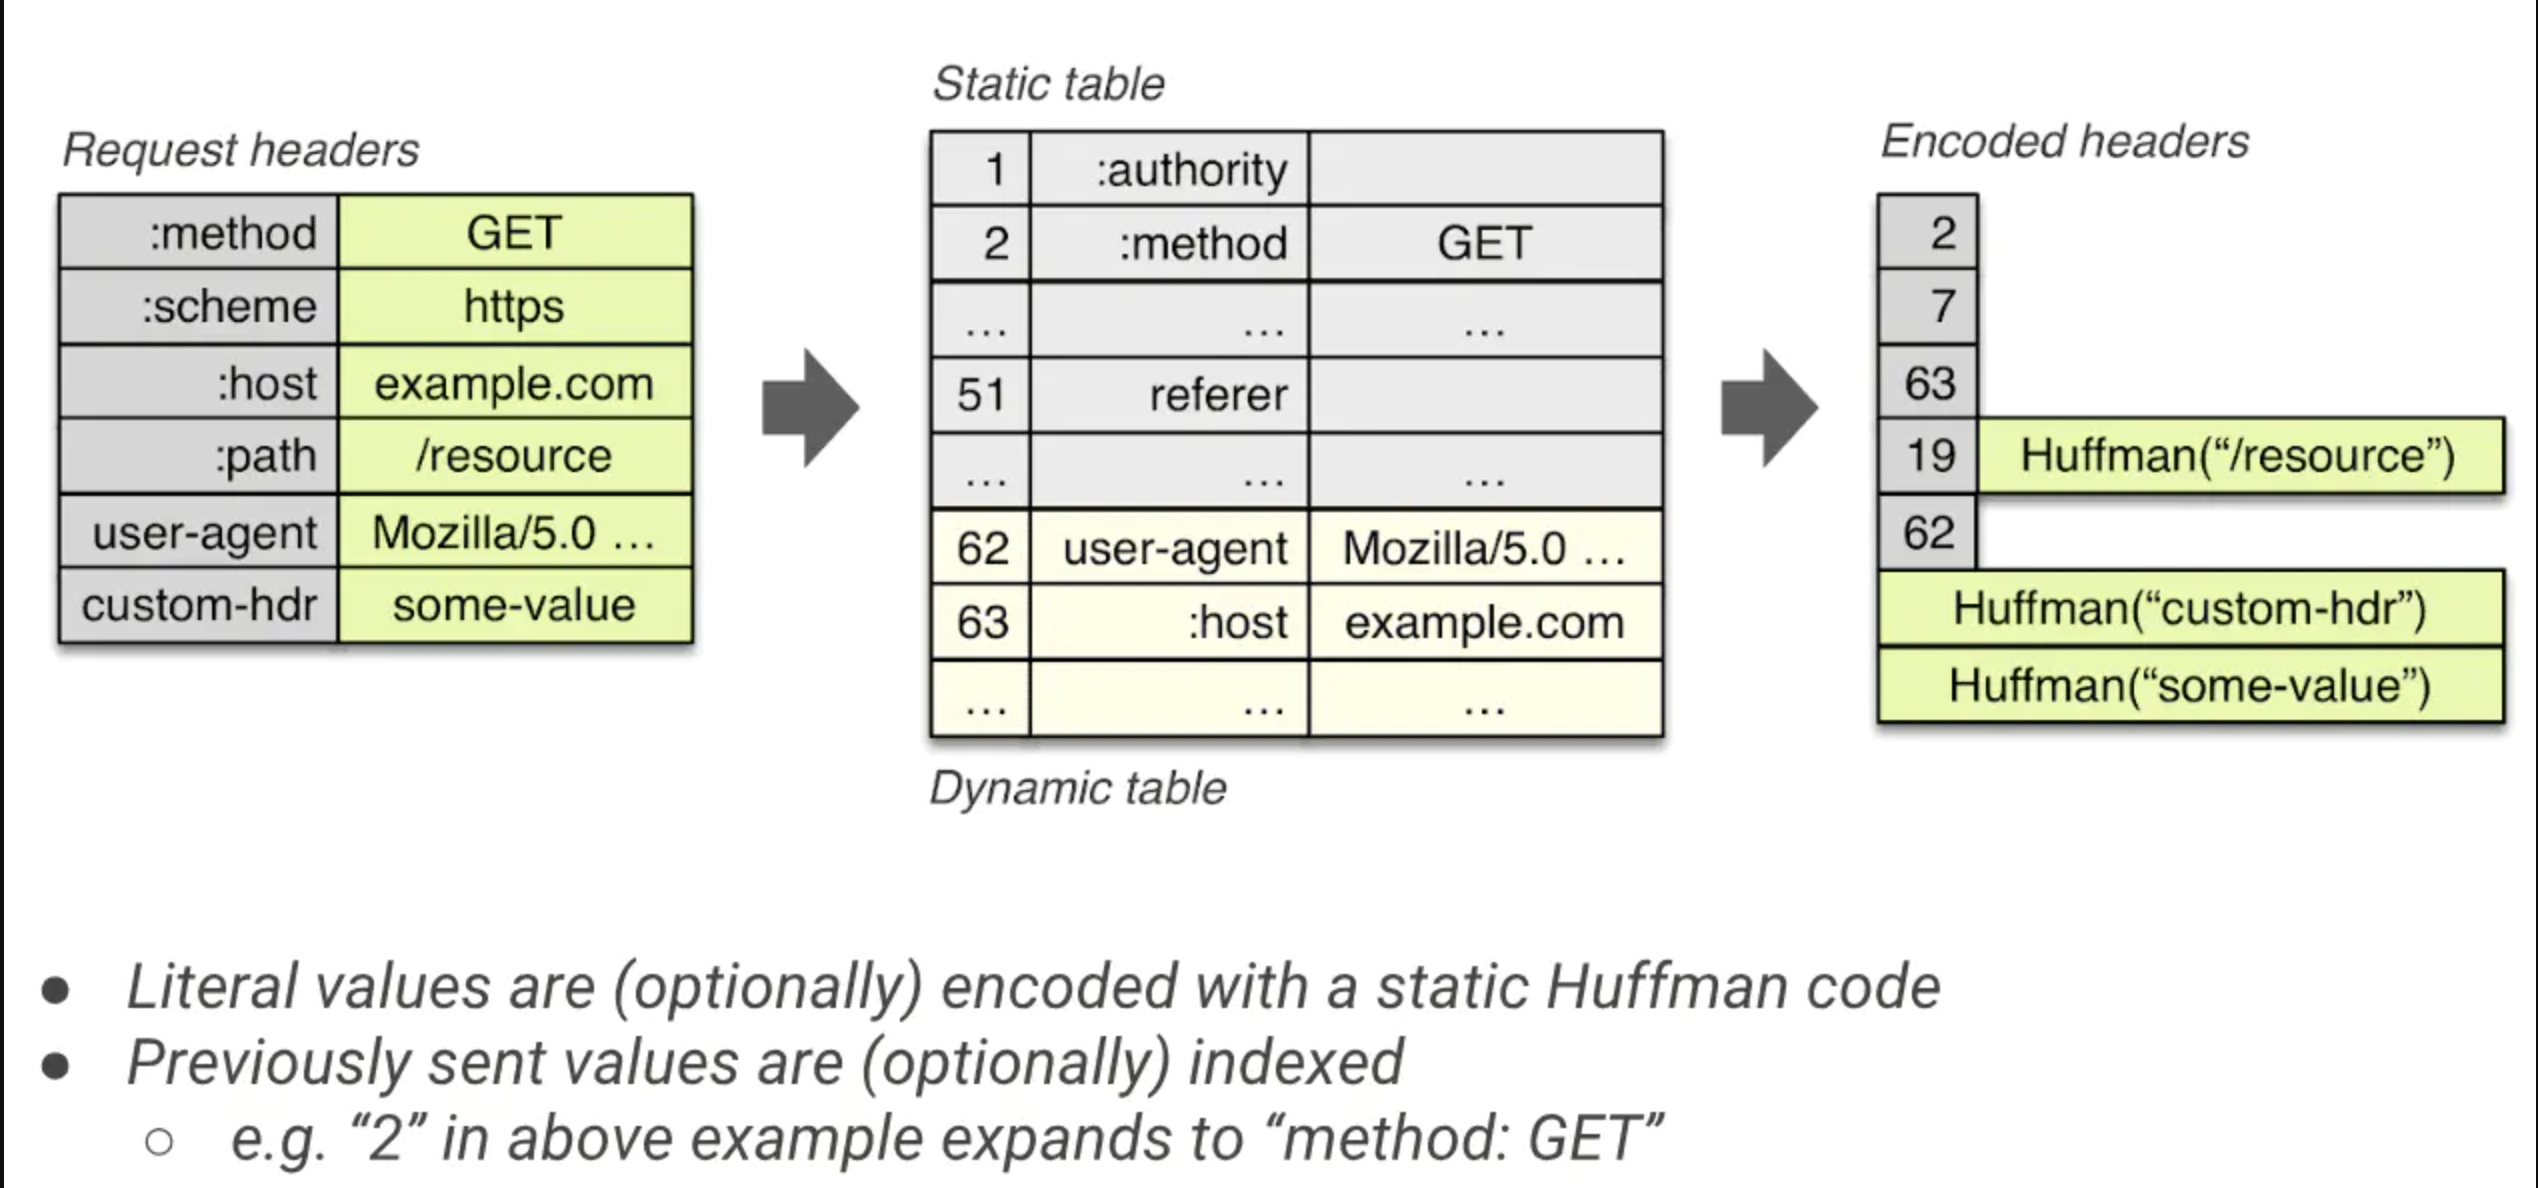
\includegraphics[width=1\textwidth]{http/http_2_hpack_get.png}
    \caption{Header压缩示例}
\end{figure}

......

\section{参考}

\href{https://tools.ietf.org/html/rfc7540}{Hypertext Transfer Protocol Version 2 (HTTP/2)} 

\href{https://tools.ietf.org/html/rfc7541}{HPACK: Header Compression for HTTP/2} 

\href{https://nghttp2.org/}{nghttp2}

\href{https://http2.golang.org/}{http2.golang}

\href{https://github.com/FiloSottile/mkcert}{mkcert}

\href{https://www.freecodecamp.org/news/how-to-get-https-working-on-your-local-development-environment-in-5-minutes-7af615770eec/}{How to get HTTPS working on your local development environment}

\href{https://http2.github.io/}{http2-spec}


《web性能权威指南》













































